% Estado técnico del MPC monolítico del SMDFR (6-11-2026).
% Compilar con XeLaTeX o LuaLaTeX (fontspec, Inter) desde docs/:
%   xelatex estado_mpc_monolitico.tex   (dos pasadas)   o   tectonic estado_mpc_monolitico.tex
% Figuras: .venv\Scripts\python python/make_status_figures.py  ->  docs/figures/
\documentclass[11pt,a4paper]{article}
\usepackage[spanish,es-noquoting,es-nodecimaldot]{babel}
\usepackage{fontspec}
% (sin UprightFont=: con Path= Tectonic no encuentra la fuente; el argumento ya es la recta)
\setmainfont[Path=../assets/fonts/,BoldFont=InterVariable.ttf,
  BoldFeatures={FakeBold=2.2},ItalicFont=InterVariable.ttf,ItalicFeatures={FakeSlant=0.15},
  BoldItalicFont=InterVariable.ttf,BoldItalicFeatures={FakeBold=2.2,FakeSlant=0.15}]{InterVariable.ttf}
\setsansfont[Path=../assets/fonts/,BoldFeatures={FakeBold=2.2}]{InterVariable.ttf}
\usepackage[margin=25mm]{geometry}
\usepackage{amsmath,amssymb,booktabs,tabularx,graphicx,array,float}
\usepackage[font=small,labelfont=bf]{caption}
\usepackage{xcolor,hyperref,enumitem}
\usepackage{tikz}
\usetikzlibrary{positioning,arrows.meta}
\definecolor{ink}{HTML}{12233B}
\definecolor{accent}{HTML}{003876}
\definecolor{soft}{HTML}{EAF5FB}
\hypersetup{colorlinks=true,linkcolor=accent,urlcolor=accent,citecolor=accent}
\setlist{itemsep=2pt,topsep=3pt}
\renewcommand{\arraystretch}{1.15}
\newcolumntype{Y}{>{\raggedright\arraybackslash}X}
\newcommand{\mdot}{\dot m}
\newcommand{\codeus}{\textunderscore\allowbreak}
\newcommand{\code}[1]{{\small\ttfamily\let\_\codeus #1}}  % nombres largos cortables en "_"
\setlength{\emergencystretch}{2em}
\newcommand{\takeaway}[1]{\par\smallskip\noindent\colorbox{soft}{\parbox{\dimexpr\linewidth-2\fboxsep}{\small #1}}\par\smallskip}
\usepackage{titlesec}
\titleformat{\section}{\large\bfseries\color{accent}}{\thesection}{0.6em}{}
\titleformat{\subsection}{\normalsize\bfseries\color{ink}}{\thesubsection}{0.6em}{}

\title{\color{accent}\bfseries MPC monolítico del SMDFR\\[2pt]
\large\mdseries Contexto, formulación, resultados y próximos pasos}
\author{Proyecto DT--SMDFR Risk Control}
\date{9 de noviembre de 2026}

\begin{document}
\maketitle

\begin{abstract}
\noindent El controlador del gemelo digital del SMDFR decidía la corriente de la bomba del
sistema de enfriamiento auxiliar (ACS) con optimizadores sin derivadas (Luus--Jaakola, GA)
que simulan el ROM en Simulink para cada candidato: minutos por consulta y resultados que
dependen de la semilla. Este documento resume la reformulación del problema como un
\emph{programa no lineal monolítico}, en el que las ecuaciones del ROM son restricciones,
y los resultados obtenidos hasta ahora:
\begin{itemize}
  \item una réplica algebraica del ROM con error de $\sim10^{-6}$~K frente a Simulink;
  \item un NLP (N3) que resuelve la consulta en $\sim0.05$~s, entre un 28 y un 56\,\%
        mejor que LJ y GA en la consulta de 1180~s;
  \item un QP linealizado (N1, N2) en forma monolítica y condensada (77 variables,
        $\sim10$~ms) con certificado dual de optimalidad global para el modelo lineal. N2,
        iterado, converge al NLP;
  \item el primer análisis de riesgo (F4) con el ensamble MC-dropout de la BiLSTM
        regenerado: está mal calibrado, pero aun así no cambia la decisión;
  \item una revisión física de las cotas del actuador: la cota en amperios no tiene
        significado físico y la autoridad la fija la rampa del actuador;
  \item la certificación del P0 no lineal (F3c). La solución es un mínimo local estricto y
        el único óptimo en $\approx590$ arranques. La primera brecha certificada es de
        2.3\,\% (1180~s) y 11.4\,\% (1161~s). Comparadas con la misma vara, N3 y N2 son las
        mejores decisiones, N1 queda a 0.0026\,\%, y LJ y GA quedan al menos un 28\,\% y un
        43\,\% por encima del óptimo global.
\end{itemize}
\end{abstract}

\section{Contexto y problema}

\paragraph{El sistema.} El SMDFR (\emph{Small Modular Dual Fluid Reactor}, 100~MWt) usa
combustible líquido y refrigerante de plomo. Caudal nominal del refrigerante:
5550.5~kg/s (Liu et al., 2021). El escenario es un LOCA de pequeña ruptura: el
refrigerante se pierde por una fuga $\mdot_{\rm leak}(t)$, el inventario $M$ baja, con
él baja el caudal primario $\mdot_c$, y la temperatura pico de vaina (PCT) sube.
Por encima de 1180~K se demanda el ACS, que repone inventario con un caudal
$\mdot_{\rm ACS}(u)$ que se fija con la corriente $u$ de una bomba MHD.

\paragraph{El gemelo digital y el controlador.} Cada 0.5~s, entre 1160 y 1190~s, un MPC
decide la secuencia de 26 acciones sobre un horizonte de 12.5~s:
\begin{itemize}
  \item el modelo de predicción es un ROM de 17 estados (Simulink);
  \item una BiLSTM con MC-dropout pronostica la fuga;
  \item un árbol dinámico de eventos (DET) representa fallas y reparaciones de los
        componentes del ACS;
  \item el costo P0 penaliza el seguimiento de la PCT a una referencia, los cambios
        bruscos de caudal y la violación del límite de 1244~K.
\end{itemize}

\paragraph{El problema.} P0 se resolvía con Luus--Jaakola (LJ) o un algoritmo genético
(GA), que tratan el ROM como una caja negra. Cada evaluación es una simulación en
Simulink, y cada consulta exige cientos de evaluaciones: unos 800~s. La acción aplicada
depende de la semilla, y no hay garantía de optimalidad. Esto impide dos cosas: volver
estocástico el MPC, que multiplica el número de escenarios, y cerrar el lazo en tiempo
real, con una meta de menos de 120~s por consulta.

\section{Plan de acción}

La idea central es escribir las ecuaciones del ROM \emph{una sola vez} en forma
algebraica. De esa única fuente salen los cuatro niveles de modelo:
\begin{itemize}
  \item N0, estado estacionario;
  \item N1, linealización en un punto (LTI);
  \item N2, linealización a lo largo de la trayectoria (LTV);
  \item N3, el modelo no lineal completo como restricciones.
\end{itemize}
El riesgo se agrega sobre esa base en tres capas de costo creciente: una restricción
probabilística analítica, escenarios (SAA) y el escenario óptimo de Homem-de-Mello et
al.~(2026).

\begin{table}[H]\centering\small
\begin{tabularx}{\linewidth}{@{}l Y Y l@{}}\toprule
Etapa & Objetivo & Criterio de cierre & Estado\\\midrule
F0 Ecuaciones & ROM escrito término a término desde el \code{.slx} & Cada término trazado a un bloque & Cerrada\\
F1 Réplica & ROM algebraico con diferenciación automática (Julia) & Error $\ll1$~K frente a Simulink & Cerrada\\
F2 NLP (N3) & P0 como NLP con JuMP + Ipopt & Comparado con LJ y GA re-simulando en Simulink & 2 consultas\\
F3 QP (N1, N2) & MPC lineal (disperso y condensado), $G(s)$, certificado dual & Brecha frente a N3 medida & 2 consultas\\
F3c Certificación & Brecha de optimalidad del P0 no lineal y comparación de decisiones & Brecha certificada pequeña & 1--4b; 4b.5 pendiente\\
F4 Riesgo & Capas probabilística, SAA y cuantiles & Una decisión que cambie por riesgo & Abierta\\
F5 Lazo cerrado & 61 consultas, multietapa & $<120$~s por consulta; frontera costo--riesgo & Pendiente\\\bottomrule
\end{tabularx}
\caption{Etapas del plan (detalle en \code{docs/monolithic\_formulation\_plan.md}).}
\end{table}

\subsection{Cómo se conectan las fases}

Las fases no son tareas independientes. Cada una produce el insumo de la siguiente y,
además, valida a la anterior. La figura~\ref{fig:fases} resume el flujo.

\begin{figure}[H]\centering
\resizebox{\linewidth}{!}{%
\begin{tikzpicture}[
  box/.style={draw=accent, line width=0.6pt, rounded corners=2pt, fill=soft,
              align=center, font=\small, minimum height=13mm, text width=24mm, inner sep=2pt},
  ref/.style={draw=black!50, dashed, rounded corners=2pt, align=center, font=\small,
              minimum height=10mm, text width=30mm},
  arr/.style={-{Stealth[length=2mm]}, line width=0.6pt, draw=ink},
  val/.style={-{Stealth[length=2mm]}, line width=0.5pt, draw=black!50, dashed},
  lab/.style={font=\footnotesize, text=black!70, align=center, inner sep=1.5pt}]
\node[box] (f0) at (0,0)      {\textbf{F0}\\Ecuaciones\\del \code{.slx}};
\node[box] (f1) at (3.6,0)    {\textbf{F1}\\Réplica\\algebraica};
\node[box] (f2) at (8.8,1.6)  {\textbf{F2}\\NLP no lineal\\(N3)};
\node[box] (f3) at (8.8,-1.6) {\textbf{F3}\\Linealización\\QP y $G(s)$};
\node[box] (f4) at (13.0,0)   {\textbf{F4}\\Riesgo\\(probab., SAA)};
\node[box] (f5) at (16.6,0)   {\textbf{F5}\\Lazo cerrado\\(61 consultas)};
\node[ref] (sim) at (3.6,-3.6) {Simulink (ROM)\\referencia exacta};
\draw[arr] (f0) -- (f1);
\draw[arr] (f1.east) -- (5.0,0) |- node[lab, pos=0.75, above]{restricciones} (f2.west);
\draw[arr] (f1.east) -- (5.0,0) |- node[lab, pos=0.75, below]{jacobianos} (f3.west);
\draw[arr] (f2) -- node[lab, right]{óptimo de\\referencia} (f3);
\draw[arr] (f2.east) -- (11.0,1.6) |- (f4.west);
\draw[arr] (f3.east) -- (11.0,-1.6) |- (f4.west);
\draw[arr] (f4) -- (f5);
\draw[val] (sim.north) -- node[lab, right]{valida} (f1.south);
\draw[val] (sim.east) -| node[lab, pos=0.3, below]{re-simula cada acción} (f3.south);
\end{tikzpicture}}
\caption{Flujo entre fases. Las flechas continuas indican qué produce cada fase para la
siguiente: F2 y F3 dan a F4 un problema tratable, y F4 da a F5 la decisión con riesgo.
Las discontinuas indican la validación contra Simulink, que se usa como
referencia exacta.}
\label{fig:fases}
\end{figure}

\begin{description}[style=nextline,leftmargin=0pt]
  \item[F0 $\to$ F1: de un diagrama a ecuaciones verificables.] El ROM vivía repartido
    en bloques de Simulink. F0 lo escribe término a término y deja trazado cada término a
    un bloque. F1 lo programa en Julia, un lenguaje con \emph{diferenciación automática},
    y lo valida contra Simulink sobre la trayectoria archivada. Sin F1 no hay derivadas
    exactas, y sin derivadas no se puede usar un optimizador basado en gradiente.
  \item[F1 $\to$ F2: el modelo pasa a ser restricción.] La réplica validada se
    escribe como restricciones de igualdad de un NLP: el nivel N3, sin aproximar nada. F2
    da el \emph{óptimo de referencia} del modelo. Contra él se mide todo lo demás: los
    optimizadores sin derivadas (LJ, GA) y las aproximaciones de F3.
  \item[F1 $\to$ F3: la misma réplica, derivada.] Los jacobianos de la réplica
    ($A,B,E$ y la salida) se obtienen por diferenciación automática, no con otro modelo.
    F3 construye con ellos el MPC lineal (un QP) y la función de transferencia, y mide su
    error contra F2. Si el error es pequeño, el modelo lineal es un sustituto legítimo.
  \item[F2, F3 $\to$ F4: el riesgo necesita un problema tratable.] Agregar
    incertidumbre multiplica el problema: por $M$ escenarios en SAA, o con una restricción
    probabilística que exige propagar distribuciones. Esto sólo es viable si el problema
    determinista es rápido (F2) y, para las capas analíticas, lineal (F3).
  \item[F4 $\to$ F5: de una consulta al lazo.] F5 resuelve el problema elegido en cada
    una de las 61 consultas, con el estado real de cada instante, y mide el costo y el
    riesgo del lazo completo.
\end{description}

\section{Fundamentos teóricos}

\subsection{Control predictivo de horizonte deslizante}
En cada instante de consulta $t_q$, el MPC resuelve un \emph{problema de control óptimo en
lazo abierto} sobre un horizonte finito de $K$ pasos, a partir del estado estimado
$\hat x(t_q)$. Aplica sólo la primera acción y repite el cálculo en $t_q+\Delta t$ con la
nueva medición. La realimentación nace de esa re-optimización: errores de modelo o de
pronóstico se corrigen en la consulta siguiente. Por eso importan dos cosas: que el
problema se resuelva en tiempo real, y que su solución sea \emph{reproducible}. Una acción
que cambia con la semilla del optimizador introduce ruido en el lazo.

\subsection{De la caja negra a la transcripción directa}
Hay dos maneras de plantear el problema de control óptimo:
\begin{itemize}
  \item \textbf{Disparo simple} (\emph{single shooting}): las únicas incógnitas son los
        controles $u_{0:K-1}$, y el costo se evalúa simulando el modelo. Es lo que hacen
        LJ y GA, que además no usan derivadas. Cada evaluación es una simulación completa,
        y la búsqueda explora a ciegas un espacio de 26 dimensiones.
  \item \textbf{Transcripción directa simultánea}: los estados $x_{0:K}$ también son
        incógnitas, y la dinámica entra como restricciones de igualdad
        $x_k=x_{k-1}+\Delta t\,f(x_k,d_k,u_k)$. El problema es más grande, pero cada
        restricción depende sólo de dos instantes consecutivos. Las matrices son
        \emph{dispersas}, las derivadas son exactas y baratas, y el optimizador no
        necesita que la trayectoria sea factible en cada iteración. Eso ayuda con
        dinámicas rígidas o inestables.
\end{itemize}
La formulación ``monolítica'' es esta segunda: simulador y optimizador quedan fusionados
en un solo problema.

\subsection{Rigidez y Euler implícito}
Los valores propios del jacobiano $A$ van desde $-1.7\cdot10^{3}$~s$^{-1}$ (la cinética
neutrónica) hasta escalas de segundos o más lentas (la termohidráulica y el inventario).
Un sistema con escalas tan separadas es \emph{rígido}. Euler explícito sería estable sólo
con $\Delta t<2/1.7\cdot10^{3}\approx1.2$~ms, unas 400 veces menor que el paso del MPC.
Euler implícito,
\[
x_k=x_{k-1}+\Delta t\,f(x_k,d_k,u_k),
\]
es A-estable y L-estable: los modos rápidos se amortiguan con cualquier $\Delta t$. Por
eso permite $\Delta t=0.5$~s. Su precisión es de primer orden. Pero como Simulink usa
\code{ode1be}, el mismo esquema, la réplica reproduce el \emph{mismo modelo discreto} y el
error de discretización es idéntico en ambos.

\subsection{Programación no lineal, condiciones KKT y punto interior}
El NLP tiene la forma $\min_z \phi(z)$ con restricciones $c(z)=0$ y $g(z)\le0$. Un óptimo
local satisface las condiciones de Karush--Kuhn--Tucker (KKT):
\[
\nabla\phi+\nabla c^\top\lambda+\nabla g^\top\mu=0,\qquad c=0,\qquad g\le0,\qquad \mu\ge0,\qquad \mu_ig_i=0 .
\]
Ipopt es un método de \emph{punto interior primal-dual}. Reemplaza las desigualdades por
una barrera logarítmica y resuelve las KKT perturbadas con pasos de Newton, que usan
primeras y segundas derivadas. JuMP las obtiene por diferenciación automática.

Como el modelo es no lineal, el problema no es convexo, y Ipopt garantiza sólo un óptimo
\emph{local}. Por eso se lanzaron cuatro inicializaciones distintas, que llegaron al mismo
óptimo. Eso es un indicio de unicidad, no una garantía. Las bisagras
$[\cdot]_+^2$ del costo original no son dos veces diferenciables. Se reescriben con
holguras ($s\ge0$, $s\ge z$, costo $s^2$), lo que es exacto y deja el problema suave.

\subsection{Linealización}
La linealización es una expansión de Taylor de primer orden de la dinámica y de la salida
alrededor de un punto $(\bar x,\bar u,\bar d)$:
\[
f(x,d,u)\approx\bar f+A(x-\bar x)+B(u-\bar u)+E(d-\bar d),\qquad
A=\frac{\partial f}{\partial x},\ B=\frac{\partial f}{\partial u},\ E=\frac{\partial f}{\partial d}.
\]
El error es de segundo orden en la distancia al punto. Por eso la calidad depende de cuánto
se aleje la trayectoria. Hay dos variantes:
\begin{itemize}
  \item \textbf{LTI (N1):} un solo punto para todo el horizonte. Es suficiente si la
        trayectoria no se aleja mucho de ese punto.
  \item \textbf{LTV (N2):} un punto por paso, $(\bar x_k,\bar u_k,\bar d_k)$, tomado de
        una trayectoria nominal no lineal. Si se itera (se linealiza, se resuelve, se
        re-simula y se vuelve a linealizar), el método es una programación cuadrática
        secuencial. Cuando converge, su punto fijo coincide con el óptimo del modelo no
        lineal.
\end{itemize}
Con la dinámica afín, el costo cuadrático y las restricciones lineales, el problema es un
\textbf{QP convexo}: todo óptimo local es global, existen métodos con tiempo de cálculo
acotado y predecible, y la dualidad entrega cotas certificadas del óptimo.

\subsection{Riesgo: restricción probabilística, SAA y dos etapas}
\begin{itemize}
  \item \textbf{Restricción probabilística.} Se exige
        $\mathbb P(\hat y_k>U_y)\le\varepsilon$. Si el modelo es lineal y el error del
        pronóstico $w$ es gaussiano, $\hat y_k=\bar y_k(u)+c_k^\top w$ también es
        gaussiano. Entonces la restricción equivale exactamente a
        \[
        \bar y_k(u)+z_{1-\varepsilon}\,\sigma_k\le U_y,\qquad \sigma_k^2=c_k^\top\Sigma c_k .
        \]
        La fuga entra de forma aditiva, así que $\sigma_k$ no depende de $u$, y la
        restricción es un \emph{ajuste lineal} de la cota: el QP sigue siendo un QP. Con el
        modelo no lineal no hay esa equivalencia.
  \item \textbf{SAA} (\emph{sample average approximation}). Reemplaza la esperanza por el
        promedio sobre $M$ escenarios muestreados. Al crecer $M$, el valor y las
        soluciones convergen a los del problema verdadero. Con $M$ finito, el óptimo dentro
        de la muestra es optimista, con sesgo hacia abajo. Por eso cada decisión se evalúa
        \emph{fuera de muestra}, con escenarios que no se usaron para optimizar.
  \item \textbf{Dos etapas y no anticipación.} La primera acción $u_0$ se decide antes de
        conocer qué escenario ocurre, así que debe ser común a todos. Las acciones
        posteriores son \emph{recurso}: pueden adaptarse a cada escenario, porque en el lazo
        se re-optimizan con información nueva. Esto evita la sobreconfianza de una
        secuencia fija en lazo abierto.
  \item \textbf{Escenario óptimo} (Homem-de-Mello et al., 2026). En programas
        estocásticos de dos etapas con segunda etapa lineal y recurso fijo, una sola
        realización bien elegida puede reproducir la decisión estocástica. En el
        \emph{newsvendor}, por ejemplo, es un cuantil de la demanda. Esto exige un modelo
        lineal y un costo en norma $L_1$: es otra razón para disponer de F3.
\end{itemize}

\section{La formulación monolítica}

\paragraph{Modelo de predicción (ROM, 17 estados).} Estado
$x=(N,C_{1..6},C^e_{1..6},T_f,T_w,T_c,\Delta M)$. Cinética puntual con precursores
circulantes y termohidráulica de tres nodos (combustible, pared y refrigerante):
\begin{gather*}
\dot N = \tfrac{\rho-\beta}{\Lambda}N+\textstyle\sum_i\lambda_iC_i,\qquad
\dot C_i = \tfrac{\beta_i}{\Lambda}N-(\lambda_i+\lambda_c)C_i+\lambda_eC^e_i,\qquad
\dot C^e_i = \lambda_cC_i-(\lambda_i+\lambda_e)C^e_i,\\
\rho = \rho_0+\alpha_f(T_f-\bar T_{f0})+\alpha_c(T_c-\bar T_{c0}),\qquad
P = \tfrac{P_0}{N_0}N,\\
M_wc_{pw}\dot T_w = h_{fw}A_{fw}(T_f-T_w)-h_{wc}(\mdot_c)A_{wc}(T_w-T_c),
\end{gather*}
con ecuaciones análogas para $T_f$ y $T_c$. El control entra sólo por el inventario:
\begin{gather*}
\dot{\Delta M}=\mdot_{\rm leak}(t)+\mdot_{\rm ACS},\qquad
\mdot_c=\mdot_{\rm nom}\frac{M_c+\Delta M}{M_c},\qquad
h_{wc}=h_{wc0}\Big(\frac{\mdot_c}{5550}\Big)^{0.8},\\
\hat y=T_w+p_4(\mdot_{\rm leak}+\mdot_{\rm ACS}+5550)+0.4,
\end{gather*}
donde $\hat y$ es la PCT estimada y $p_4$ es una regresión de grado 4 del desvío entre el
HRM y el ROM.

\paragraph{P0 como NLP.} La decisión pasa a ser el caudal $\mdot_{\rm ACS}$, y la
corriente se recupera con el mapa inverso de la bomba. La dinámica se impone con Euler
implícito, igual que el integrador \code{ode1be} de Simulink. Las bisagras
$[\cdot]_+^2$ del costo se reemplazan por holguras, lo que es exacto:
\begin{align*}
\min_{\mdot,\,x,\,s,\,r}\quad & \sum_{k=1}^{K}(\hat y_k-y_{\rm ref})^2+\lambda_m\sum_k s_k^2+\lambda_{\rm pct}\sum_k r_k^2\\
\text{s.a.}\quad & x_k=x_{k-1}+\Delta t\,f(x_k,\hat d_k,\mdot_k),\quad x_0=\hat x(t_q-\Delta t),\\
& |\mdot_{k+1}-\mdot_k|\le\Delta\mdot+s_k,\qquad \hat y_k-U_y\le r_k,\qquad s,r\ge0,\qquad
\mdot_{\rm min}\le\mdot_k\le\mdot_{\rm max},
\end{align*}
con $K=26$, $\Delta t=0.5$~s, $U_y=1244$~K, $\lambda_m=10^{-4}$, $\Delta\mdot=5$~kg/s y
$\lambda_{\rm pct}=10$, los valores de \code{fitness\_cost.m}. El problema tiene unas
520 variables libres (442 de estado, 26 de control y 51 holguras) y 442 restricciones de
dinámica.

\emph{Escalado.} $N\sim10^{13}$ y $C_i\sim10^{16}$ conviven con temperaturas de
$\sim10^3$~K. Por eso cada estado se escribe como $x_j=S_jz_j$, con
$S_j=\max(|x_{j,0}|,1)$. Sin este cambio, las matrices de Newton quedan mal
condicionadas y Ipopt no converge de forma fiable.

\paragraph{Niveles del modelo.} Este NLP es el nivel N3. Los niveles linealizados N1 y
N2, cómo se resuelve cada uno y para qué sirven se detallan en la
sección~\ref{sec:niveles}.

\paragraph{Riesgo (F4): SAA en dos etapas.} Con $M$ trayectorias $\hat d^{(j)}$ de fuga
del ensamble MC-dropout, la primera acción $\mdot_0$ es común a todos los escenarios y el
resto del horizonte es un recurso por escenario:
\[
\min_{\mdot_0}\ \frac1M\sum_{j=1}^{M}\ \min_{\mdot_{1:K-1}^{(j)}} J_{\rm P0}\big(\mdot_0,\mdot^{(j)}_{1:K-1};\hat d^{(j)}\big).
\]
Es la estructura de dos etapas que supone el teorema del escenario óptimo.

\section{Los tres niveles del modelo: N3, N1 y N2}\label{sec:niveles}

Los tres niveles resuelven \emph{el mismo} problema P0, con el mismo costo y las mismas
restricciones sobre el actuador. Lo único que cambia es cómo se representa la dinámica
$x_k=x_{k-1}+\Delta t\,f(x_k,d_k,u_k)$ en las restricciones.

\begin{figure}[H]\centering
\resizebox{\linewidth}{!}{%
\begin{tikzpicture}[
  curve/.style={line width=1.2pt, draw=accent},
  tang/.style={line width=0.9pt, draw=orange!85!black},
  pt/.style={circle, fill=orange!85!black, inner sep=1.4pt},
  ttl/.style={font=\small\bfseries, text=ink},
  sub/.style={font=\scriptsize, text=black!65, align=center}]
\begin{scope}
  \draw[black!40, ->] (0,0) -- (4.2,0) node[below left, sub]{$x$};
  \draw[black!40, ->] (0,0) -- (0,3) node[below left, sub, rotate=90]{$f(x)$};
  \draw[curve] (0.2,0.4) .. controls (1.5,0.5) and (2.6,1.4) .. (4,2.8);
  \draw[tang] (0.2,0.42) -- (4,1.25);
  \node[pt] at (0.7,0.53) {};
  \node[ttl] at (2.1,3.3) {N1 (LTI)};
  \node[sub] at (2.1,-0.55) {una tangente en el punto de consulta,\\válida en todo el horizonte};
\end{scope}
\begin{scope}[xshift=5.6cm]
  \draw[black!40, ->] (0,0) -- (4.2,0) node[below left, sub]{$x$};
  \draw[black!40, ->] (0,0) -- (0,3) node[below left, sub, rotate=90]{$f(x)$};
  \draw[curve] (0.2,0.4) .. controls (1.5,0.5) and (2.6,1.4) .. (4,2.8);
  \foreach \x/\y/\s in {0.7/0.53/0.25, 1.6/0.82/0.45, 2.5/1.33/0.75, 3.4/2.08/0.95}
    { \draw[tang] ({\x-0.42},{\y-0.42*\s}) -- ({\x+0.42},{\y+0.42*\s}); \node[pt] at (\x,\y) {}; }
  \node[ttl] at (2.1,3.3) {N2 (LTV, iterado)};
  \node[sub] at (2.1,-0.55) {una tangente por paso $k$, en la trayectoria\\del incumbente; se re-linealiza cada iteración};
\end{scope}
\begin{scope}[xshift=11.2cm]
  \draw[black!40, ->] (0,0) -- (4.2,0) node[below left, sub]{$x$};
  \draw[black!40, ->] (0,0) -- (0,3) node[below left, sub, rotate=90]{$f(x)$};
  \draw[curve] (0.2,0.4) .. controls (1.5,0.5) and (2.6,1.4) .. (4,2.8);
  \node[ttl] at (2.1,3.3) {N3 (no lineal)};
  \node[sub] at (2.1,-0.55) {la dinámica exacta como restricción;\\sin aproximación};
\end{scope}
\end{tikzpicture}}
\caption{Esquema de los tres niveles. La curva azul representa la dinámica no lineal $f$,
y en naranja están las aproximaciones lineales. N1 usa una sola tangente; N2, una por
paso del horizonte, que se actualizan en cada iteración; N3 usa la curva misma.}
\end{figure}

\subsection{N3: el modelo no lineal completo}
Es el NLP de la sección anterior. Ipopt lo resuelve con pasos de Newton sobre las KKT
perturbadas por la barrera. Usa la matriz hessiana exacta del lagrangiano, que JuMP
obtiene por diferenciación automática, y tarda unos 0.05~s. El problema no es convexo, así
que el resultado es un óptimo \emph{local}, sin certificado de optimalidad global.

\subsection{N1: un solo punto de linealización (LTI)}
Se linealiza una vez, en $(\bar x,\bar d,\bar u)=(x(t_q-\Delta t),\ d(t_q-\Delta t),\
\tfrac12(\mdot_{\rm min}+\mdot_{\rm max}))$. Las matrices $A$, $B$, $E$ y $D$ son las
mismas para los 26 pasos. Conviene escribir el modelo en \emph{desviaciones},
$\delta_k=x_k-\bar x_k$, $\Delta u_k=u_k-\bar u_k$ y $\Delta d_k=d_k-\bar d_k$, porque así
se evita restar números de $\sim10^{16}$ (ver los resultados de F3). Con Euler implícito:
\begin{gather*}
(I-\Delta t\,A_k)\,\delta_k=\delta_{k-1}+r_k+\Delta t\,B_k\,\Delta u_k+\Delta t\,E_k\,\Delta d_k,
\qquad r_k=\bar x_{k-1}-\bar x_k+\Delta t\,\bar f_k,\\
\hat y_k=\bar y_k+\delta_{k}[T_w]+D_k\,(\Delta d_k+\Delta u_k),
\end{gather*}
con $A_k\equiv A$ en N1, $\bar x_k\equiv\bar x$ y, por lo tanto, $r_k=\Delta t\,\bar f$.
Con este modelo, P0 es un QP convexo: costo cuadrático en $\hat y$, que es afín en $u$, y
restricciones lineales.

\subsection{N2: un punto por paso, actualizado por programación secuencial (LTV)}
\paragraph{Dos índices.} En N2 conviven dos índices que no hay que confundir:
\begin{itemize}
  \item $k=1,\dots,26$ es el paso del horizonte de predicción;
  \item $i=1,2,\dots$ es la iteración de la programación secuencial.
\end{itemize}
En la iteración $i$, los jacobianos del paso $k$ se evalúan en el estado $\bar x_k^{(i-1)}$,
en el \emph{mismo paso} $k$, de la trayectoria no lineal que produce el control incumbente
$u^{(i-1)}$ de la iteración anterior:
\[
A_k^{(i)}=\frac{\partial f}{\partial x}\Big(\bar x_k^{(i-1)},d_k,u_k^{(i-1)}\Big),\quad
B_k^{(i)}=\frac{\partial f}{\partial u}(\cdot),\quad
E_k^{(i)}=\frac{\partial f}{\partial d}(\cdot),\qquad
\bar x^{(i-1)}=\mathcal S\big(x_0,\,u^{(i-1)},\,d\big),
\]
donde $\mathcal S$ es la simulación no lineal (la réplica). No dependen del paso $k-1$ de
la misma iteración: los 26 jacobianos se calculan juntos, a partir de una trayectoria ya
simulada, \emph{antes} de resolver el QP. La matriz del paso $k$ cambia con $k$ porque la
trayectoria nominal recorre estados distintos (el inventario crece y la PCT baja), y cambia
con $i$ porque la trayectoria se corrige en cada iteración.

\begin{figure}[H]\centering
\resizebox{0.92\linewidth}{!}{%
\begin{tikzpicture}[
  st/.style={draw=accent, line width=0.6pt, rounded corners=2pt, fill=soft, align=center,
             font=\small, minimum height=14mm, text width=40mm},
  arr/.style={-{Stealth[length=2mm]}, line width=0.6pt, draw=ink},
  lab/.style={font=\footnotesize, text=black!70, align=center}]
\node[st] (a) at (0,0)    {\textbf{1. Simular} la réplica\\con el incumbente $u^{(i-1)}$:\\$\bar x^{(i-1)}_{1..K}$};
\node[st] (b) at (5.2,0)  {\textbf{2. Linealizar} en cada\\paso $k$: $A_k^{(i)}, B_k^{(i)}, E_k^{(i)}$\\(ForwardDiff)};
\node[st] (c) at (10.4,0) {\textbf{3. Resolver el QP}\\convexo (Clarabel):\\$u^{(i)}$};
\node[st] (d) at (10.4,-2.5) {\textbf{4. ¿Convergió?}\\$\|u^{(i)}-u^{(i-1)}\|_\infty<\epsilon$};
\node[st, fill=white] (e) at (5.2,-2.5) {\textbf{Fin:} $u^\star=u^{(i)}$\\(punto KKT de N3)};
\draw[arr] (a) -- (b); \draw[arr] (b) -- (c); \draw[arr] (c) -- (d);
\draw[arr] (d) -- node[lab, above]{sí} (e);
\draw[arr] (d.south) -- ++(0,-0.55) -| node[lab, pos=0.25, below]{no: $i\leftarrow i+1$} (a.south);
\end{tikzpicture}}
\caption{Iteración de N2. Cada vuelta usa el modelo exacto sólo para simular y derivar, y
optimiza sobre un QP convexo.}
\end{figure}

\noindent Este esquema es una \emph{programación cuadrática secuencial} sin término de
curvatura de las restricciones. También es análogo al LQR iterativo. Si converge, el punto
fijo cumple las condiciones KKT del NLP (N3): en ese punto, el modelo lineal y el no lineal
tienen el mismo valor y las mismas primeras derivadas. N1 equivale a detenerse en la
primera iteración con un punto constante.

\subsection{Cómo se resuelven los QP: forma dispersa y forma condensada}
\begin{itemize}
  \item \textbf{Monolítica dispersa.} Los estados $\delta_{1..K}$ son variables y la
        dinámica lineal son restricciones de igualdad: es la misma transcripción directa
        del NLP, con la dinámica afín. Tiene 519 variables y 442 igualdades de estructura
        bloque-bidiagonal (figura~\ref{fig:estructura}, izquierda).
  \item \textbf{Condensada.} Los estados se eliminan con la recursión anterior:
        $\delta_k=(I-\Delta t A_k)^{-1}\big(\delta_{k-1}+r_k+\Delta tB_k\Delta u_k+\Delta tE_k\Delta d_k\big)$.
        La salida queda como una función afín del control, $\hat y=\hat y^{0}+G\,u$, con
        $G\in\mathbb R^{26\times26}$ triangular inferior. La triangularidad expresa la
        causalidad: $u_j$ sólo afecta a $\hat y_k$ con $k\ge j$. Las columnas de $G$ son
        casi constantes bajo la diagonal: es la huella del integrador del inventario. Quedan
        77 variables: 26 controles y las holguras de las bisagras.
\end{itemize}
Ambas formas dan la misma solución. La condensada es más pequeña y densa. Es la base de un
MPC explícito o embebido, y con Clarabel se resuelve en unos 10~ms.

\paragraph{Certificado de optimalidad (dualidad).} Para un QP convexo
$\min\{\tfrac12z^\top Pz+q^\top z:\ Az\le b,\ Fz=g\}$, la función dual $g(\lambda,\nu)$
cumple la dualidad débil: $g(\lambda,\nu)\le p^\star$ para todo $\lambda\ge0$. Bajo
condiciones de Slater hay dualidad fuerte, $g^\star=p^\star$. Un solver primal-dual como
Clarabel entrega un par $(z,\lambda,\nu)$, y la \textbf{brecha dual}
$p(z)-g(\lambda,\nu)\ge0$ acota cuánto puede mejorarse la solución: es un
\emph{certificado de optimalidad global}. Hay que entender bien qué certifica: el óptimo
del \emph{modelo lineal} (N1 o N2), no el del P0 no lineal. Para certificar N3 hace falta
acotar el error de linealización: eso se hizo en F3c (sección~\ref{sec:f3c}).

\paragraph{Para qué sirven N1 y N2.} No buscan reemplazar al NLP, que ya es rápido. Buscan
abrir lo que el modelo no lineal no permite:
\begin{enumerate}
  \item \textbf{Garantías.} Un QP convexo da el óptimo global de su modelo, con tiempo de
        cálculo acotado y un certificado dual, ya calculado para N1 y N2 (sección~\ref{sec:f3}).
  \item \textbf{Riesgo analítico.} Bajo linealidad, un error gaussiano sigue siendo
        gaussiano. La restricción probabilística se vuelve un ajuste lineal de la cota y el
        problema sigue siendo un QP (capa 1). Con $M$ escenarios, el SAA es un QP con
        estructura de bloques (capa 2), y el teorema del escenario óptimo exige un modelo
        lineal (capa 3).
  \item \textbf{Comprensión física.} La función de transferencia
        $G(s)=C(sI-A)^{-1}B+D$, de $\mdot_{\rm ACS}$ a $\hat y$, muestra que el actuador
        actúa a través de un integrador puro (el inventario). Eso explica la estructura
        ``saturar y luego seguir'' y la autoridad limitada del ACS.
  \item \textbf{Medir la no linealidad.} La diferencia entre N1 y N3 cuantifica cuánto
        importa la no linealidad en el horizonte para la decisión.
\end{enumerate}

\section{Resultados}

\subsection{F1: la réplica algebraica reproduce Simulink}

\begin{figure}[H]\centering
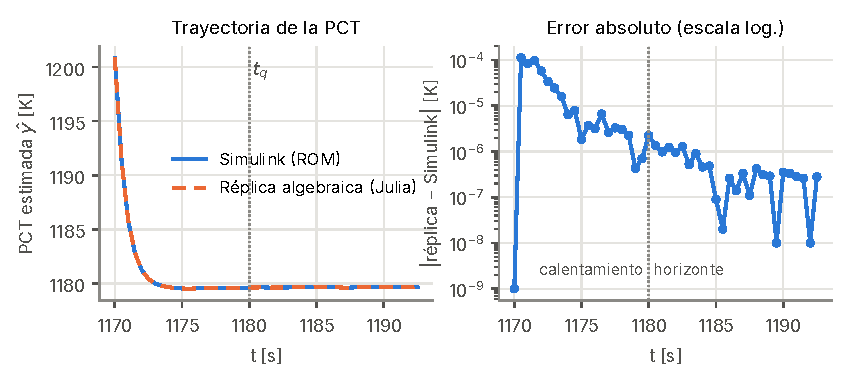
\includegraphics[width=\linewidth]{figures/fig_replica.pdf}
\caption{Consulta $t_q=1180$~s. La simulación arranca en $t_q-10$~s con el estado
inyectado desde el HRM: 10~s de calentamiento y luego el horizonte. La réplica en Julia
(\code{ode1be} con una iteración de Newton y entradas en $t_{n+1}$) sigue a Simulink con
un error de $2\cdot10^{-6}$~K en el horizonte y de $10^{-4}$~K en el transitorio del
calentamiento.}
\end{figure}

\subsection{F2: el NLP monolítico frente a los optimizadores sin derivadas}

\begin{figure}[H]\centering
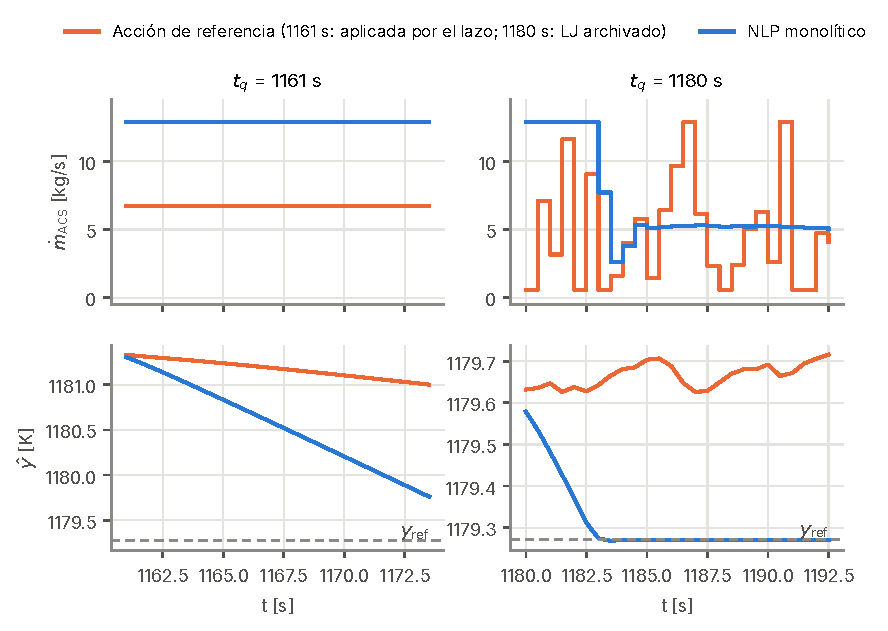
\includegraphics[width=\linewidth]{figures/fig_f2_nlp.pdf}
\caption{Acción (arriba) y PCT estimada (abajo) en las dos consultas, con la cota
archivada $u\le56.75$~A ($\mdot\le12.86$~kg/s). En 1180~s el NLP satura durante 3~s para
bajar la PCT y luego sigue la referencia exactamente. En 1161~s, la fase aguda, el óptimo
es la esquina $u=u_{\rm max}$ durante todo el horizonte, y aun así la PCT no alcanza la
referencia.}
\end{figure}

\begin{figure}[H]\centering
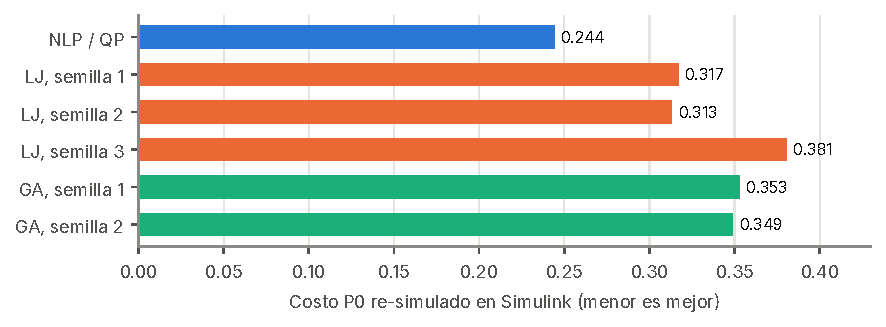
\includegraphics[width=\linewidth]{figures/fig_e2.pdf}
\caption{Consulta de 1180~s: costo P0 de cada acción re-simulada en Simulink con el mismo
evaluador (\code{DET\_2} + \code{fitness\_cost}). LJ corregido usa 721 evaluaciones y
unos 830~s; GA, 420 evaluaciones y unos 615~s; el NLP, 0.1~s. El LJ archivado, anterior
a la corrección de la búsqueda, costaba 4.08 y queda fuera de escala.}
\end{figure}

\takeaway{\textbf{Lectura.} Ningún optimizador sin derivadas alcanza el óptimo: quedan
entre un 28 y un 56\,\% por encima, y en 2 de 5 corridas la primera acción, que es la que
se aplica, no satura. El NLP y el QP dan siempre la misma acción y son unas $10^4$ veces
más rápidos. Las cuatro inicializaciones del NLP llegan al mismo óptimo. En temperatura
las diferencias son pequeñas, con un máximo de 0.02~K de PCT, así que en esta consulta el
beneficio es velocidad y reproducibilidad.}

\subsection{F3: N1 y N2 frente a N3, certificados y forma condensada}\label{sec:f3}

\paragraph{Trayectorias de control.} La figura~\ref{fig:nlpqp} superpone las trayectorias
completas, no sólo la primera acción. En 1161~s las tres saturan durante todo el horizonte
y coinciden a $10^{-7}$~kg/s. En 1180~s, N1 se separa del NLP hasta 0.054~kg/s, justo
donde el óptimo deja la saturación ($t\approx1183$~s): es el error de usar una sola
tangente. N2 converge al NLP a $6\cdot10^{-6}$~kg/s. La primera acción, que es la que se
aplica, coincide en todos los casos a $\le2\cdot10^{-5}$~kg/s.

\begin{figure}[H]\centering
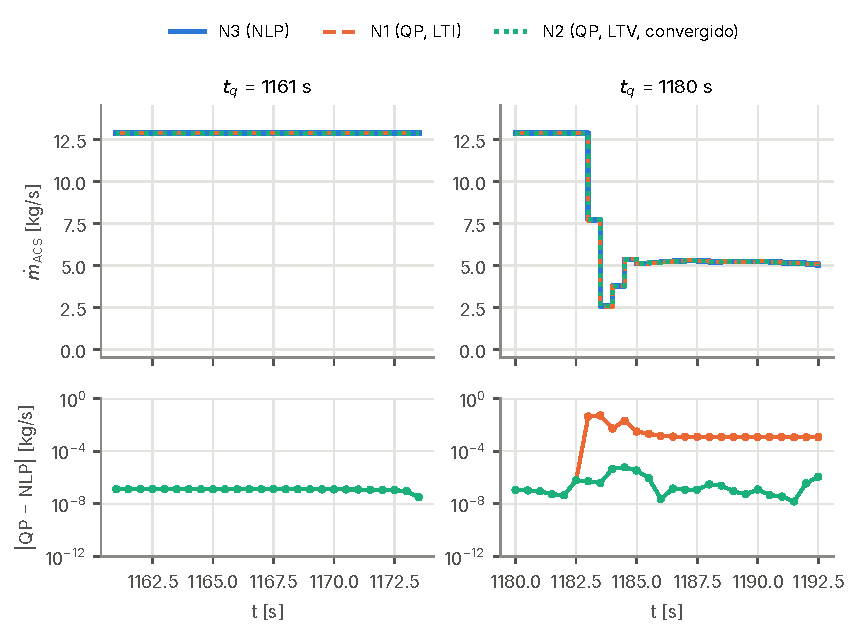
\includegraphics[width=\linewidth]{figures/fig_nlp_vs_qp.pdf}
\caption{Arriba, las acciones de N3 (NLP), N1 y N2 (convergido). Abajo, la diferencia
absoluta con el NLP en escala logarítmica.}
\label{fig:nlpqp}
\end{figure}

\begin{figure}[H]\centering
\begin{minipage}{0.56\linewidth}
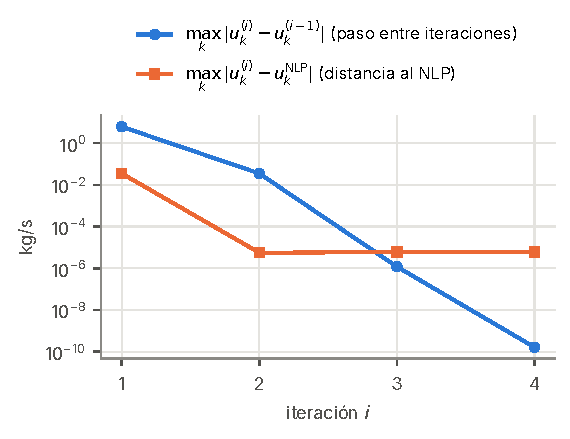
\includegraphics[width=\linewidth]{figures/fig_sqp.pdf}
\end{minipage}\hfill
\begin{minipage}{0.4\linewidth}\small
\captionof{figure}{Convergencia de N2 en $t_q=1180$~s. El paso entre iteraciones cae de
forma superlineal (6.1, $3.5\cdot10^{-2}$, $1.2\cdot10^{-6}$, $1.6\cdot10^{-10}$~kg/s), y
la distancia al NLP se estabiliza en $6\cdot10^{-6}$~kg/s, el nivel de tolerancia del
propio NLP. En 1161~s converge en una iteración.}
\end{minipage}
\end{figure}

\paragraph{Solvers, formas y certificados.} Cada QP se resolvió en sus dos formas, con
Ipopt (un solver general de NLP) y con Clarabel (un solver cónico primal-dual que entrega
la brecha dual):

\begin{table}[H]\centering\footnotesize\setlength{\tabcolsep}{4pt}
\begin{tabular}{@{}llrrrrr@{}}\toprule
Modelo & Forma, solver & Var. & Tiempo [s] & Brecha dual & $\max_k|u_k-u^{\rm NLP}_k|$ [kg/s] & Costo re-sim.\\\midrule
\multicolumn{7}{@{}l}{\emph{$t_q=1180$~s}}\\
N3 & disperso, Ipopt & 519 & 0.055 & --- & --- & 0.2439975\\
N1 & disperso, Ipopt & 519 & 0.037 & --- & $5.4\cdot10^{-2}$ & 0.2440038\\
N1 & disperso, Clarabel & 519 & 0.037 & $1.4\cdot10^{-12}$ & $5.4\cdot10^{-2}$ & 0.2440038\\
N1 & condensado, Clarabel & 77 & 0.010 & $4.3\cdot10^{-12}$ & $5.4\cdot10^{-2}$ & 0.2440038\\
N2 & disperso, Clarabel & 519 & 0.053 & $<10^{-11}$ & $5.9\cdot10^{-6}$ & 0.2439975\\
N2 & condensado, Clarabel & 77 & 0.010 & $<10^{-11}$ & $5.9\cdot10^{-6}$ & 0.2439975\\
\multicolumn{7}{@{}l}{\emph{$t_q=1161$~s}}\\
N3 & disperso, Ipopt & 519 & 0.048 & --- & --- & 48.026943\\
N1 & condensado, Clarabel & 77 & 0.009 & $4.0\cdot10^{-11}$ & $1.3\cdot10^{-7}$ & 48.026944\\
N2 & condensado, Clarabel & 77 & 0.009 & $3.9\cdot10^{-11}$ & $1.3\cdot10^{-7}$ & 48.026944\\\bottomrule
\end{tabular}
\caption{Las filas de N2 corresponden al QP linealizado en el punto fijo. Su tiempo es el
de un QP; cada iteración agrega la simulación y los jacobianos. Ipopt no entrega valor
dual. Las tablas completas están en \code{results/f3\_certificates/}.}
\end{table}

\begin{figure}[H]\centering
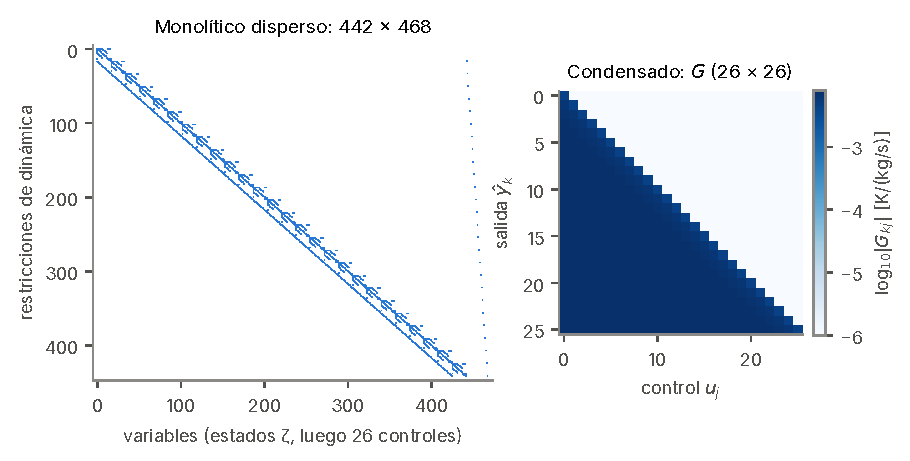
\includegraphics[width=\linewidth]{figures/fig_structure.pdf}
\caption{Estructura del QP de N1 en 1180~s. A la izquierda, la matriz de restricciones de
la forma monolítica dispersa: bloques $(I-\Delta tA)$ en la diagonal, $-I$ en la
subdiagonal y una columna por control. A la derecha, la matriz condensada $G$: triangular
inferior por causalidad, con columnas casi constantes por el integrador del inventario.}
\label{fig:estructura}
\end{figure}

\takeaway{\textbf{Lectura.} (i) \textbf{Hay certificado para el modelo lineal:} Clarabel
cierra la brecha dual a $\sim10^{-12}$, lo que demuestra que la solución de N1 y de N2 es
el óptimo global de su QP. El certificado del P0 no lineal requiere acotar además el error
de linealización (sección~\ref{sec:f3c}). (ii) El punto fijo de N2 es un punto factible de N3 con el
mismo costo que el óptimo de Ipopt (diferencia de $4\cdot10^{-8}$). Es una verificación
independiente del óptimo local del NLP. (iii) La forma condensada reduce el problema de
519 a 77 variables y el tiempo a $\sim10$~ms. (iv) El óptimo es \emph{plano}: N1 se aleja
0.054~kg/s del NLP y su costo re-simulado sólo sube un 0.0026\,\%.}

\paragraph{Corrección respecto de la versión anterior de F3.} La implementación original
(\code{f3\_linearized\_qp.jl}) hacía que N2 se estancara a 0.020~kg/s del NLP. Se probó la
hipótesis de que la causa era linealizar sobre trayectorias \code{ode1be} en lugar de
Euler implícito convergido, y quedó \textbf{descartada}: con la formulación en
desviaciones, ambas variantes dan las mismas iteraciones y convergen al NLP. La causa
estaba en la implementación anterior, que escribía el modelo afín con los términos
constantes $\bar f-A\bar x$, con $C_i\sim10^{16}$. No se aisló el detalle exacto. La
versión nueva es \code{f3\_certificates\_condensed.jl}.

\paragraph{Función de transferencia.} La función de transferencia de $\mdot_{\rm ACS}$ a
$\hat y$ explica la forma de la solución. El caudal del ACS actúa a través del inventario, que es un integrador puro:
$G(s)\approx G_M/s$, con $\partial\hat y/\partial\Delta M=-1.6\cdot10^{-2}$~K/kg. Por eso
conviene acumular inventario lo antes posible ("saturar y luego seguir"). Con la cota
archivada, la autoridad sobre el horizonte es de unos 150~kg, es decir $\approx-2.4$~K
como máximo sobre la PCT.

\subsection{F4: el riesgo del pronóstico de fuga}

\paragraph{Ensamble regenerado.} La ventana de entrada de la BiLSTM (200 muestras de fuga y
de $T_{e,c}$) se reconstruyó desde las trayectorias archivadas, con los pesos
\code{model\_200x200\_drop1\_1.pth}. La muestra archivada en 1180~s cae dentro
del ensamble regenerado. Además se halló que el lazo archivado usaba \code{N\_par = 1}:
el MPC decidía con \emph{una} realización aleatoria del dropout.

\begin{figure}[H]\centering
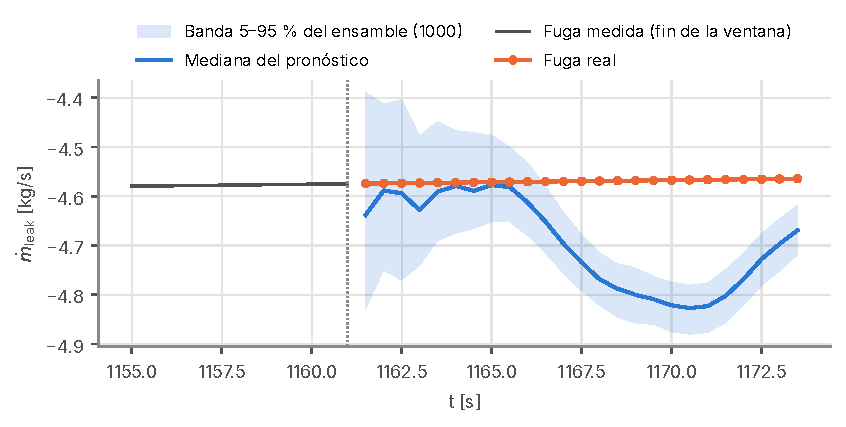
\includegraphics[width=\linewidth]{figures/fig_forecast.pdf}
\caption{Pronóstico de la fuga en $t_q=1161$~s. La fuga real (registrada en el HRM) queda
en el borde superior de la banda del 90\,\% o fuera de ella.}
\end{figure}

\begin{figure}[H]\centering
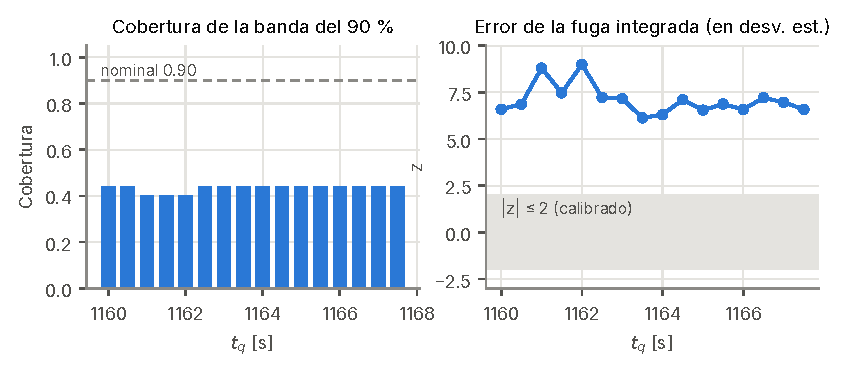
\includegraphics[width=\linewidth]{figures/fig_calibration.pdf}
\caption{Calibración en 16 consultas (1160--1167.5~s), con 500 trayectorias cada una. La
banda del 90\,\% cubre la fuga real el 44\,\% de las veces, y el error de la fuga
integrada sobre el horizonte es de unas 7 desviaciones estándar del ensamble.}
\end{figure}

\noindent El pronóstico está \textbf{sesgado}: la fuga real es unos 0.12~kg/s menor en
magnitud. También es \textbf{sobreconfiado}: el error de la mediana (0.16~kg/s) duplica
la dispersión del ensamble (0.08~kg/s). Sin embargo, ese error, integrado en el horizonte
(1.5~kg), equivale a sólo $\approx0.025$~K de PCT, y la dispersión del ensamble a
$\approx0.003$~K.

\begin{table}[H]\centering\small
\begin{tabularx}{\linewidth}{@{}Y ll@{}}\toprule
& $t_q=1161$~s & $t_q=1180$~s\\\midrule
$u_0$ con fuga p05, p50, p95, sin dropout, real y SAA-59 & todas 56.750~A & todas 56.750~A\\
Costo medio fuera de muestra (941 miembros), rango entre variantes & 48.350 (idéntico) & 0.2443--0.2480\\
Tiempo: NLP determinista / SAA con 59 escenarios & 0.03~s / 2.2~s & 0.03~s / 2.3~s\\\bottomrule
\end{tabularx}
\caption{Ninguna variante del riesgo de pronóstico cambia la primera acción.}
\end{table}

\subsection{Cotas del actuador con base física}

Las conclusiones anteriores usan la cota archivada $u\in[56.69,56.75]$~A. Al revisarla
aparecieron tres hechos:
\begin{itemize}
  \item El ACS es una \emph{inyección de reposición de inventario}; el caudal primario es
        consecuencia del inventario.
  \item En las consultas ya se perdió el 40\,\% del inventario (unos 3300~kg), y
        $\mdot_c\approx0.6\,\mdot_{\rm nom}$. La banda exploratoria de $\pm20$\,\% sobre
        el caudal nominal ya está violada por el propio LOCA. Recuperar
        $0.8\,\mdot_{\rm nom}$ exigiría unos 1700~kg, lo que no cabe en un horizonte de
        12.5~s.
  \item El ECM de la bomba es el de una \emph{bomba principal}: ducto de
        $0.515\times0.515$~m, 15~kPa, 5543~kg/s a 2~m/s. El ACS usa el pie de su curva:
        0--13~kg/s en 0.06~A, con 1~mA equivalente a 0.2~kg/s. La cota en amperios no
        tiene significado físico; la cota defendible está en kg/s.
\end{itemize}

\begin{figure}[H]\centering
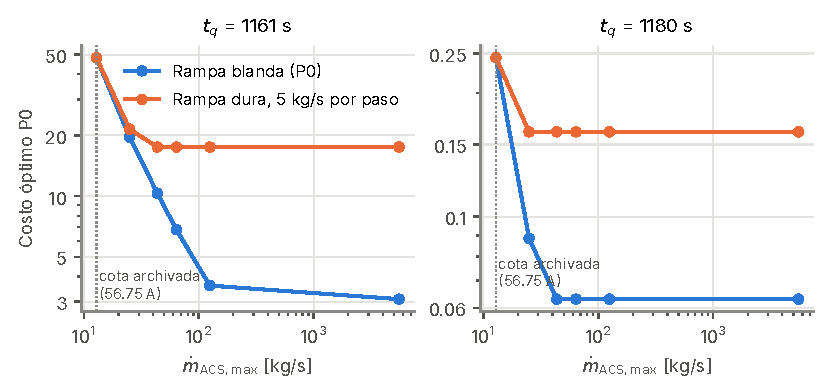
\includegraphics[width=\linewidth]{figures/fig_actuator.pdf}
\caption{Costo óptimo según la cota de caudal $\mdot_{\rm ACS,max}$, con la rampa blanda
de P0 (penalización con $\lambda_m=10^{-4}$) o con una rampa dura de 5~kg/s por paso
(10~kg/s$^2$) desde la acción aplicada.}
\end{figure}

\takeaway{\textbf{Lectura.} Con la rampa dura, la cota de caudal deja de importar desde
25--44~kg/s: la autoridad la fija la rampa. La pregunta física pasa de ``¿qué $u_{\rm max}$?''
a ``¿qué rampa admite la inyección?''. Con la rampa blanda, el óptimo deja de saturar sobre
unos 40~kg/s en 1180~s y unos 170~kg/s en 1161~s. Aun entonces, decidir con p05 o p95 mueve
$\mdot_0$ como mucho 0.5~kg/s, y fuera de muestra cuesta un 5--6\,\% más que el SAA en
1180~s. La conclusión de F4 se mantiene: la incertidumbre de pronóstico de la fuga no
cambia la decisión de forma relevante. El polinomio $p_4$ se extrapola en estos casos,
pero su aporte es de 0.017~K como máximo.}

\section{Certificación de optimalidad del P0 no lineal (F3c)}\label{sec:f3c}

\subsection{Qué se quiere certificar}
El problema de referencia es P0 sobre el ROM \textbf{no lineal} (N3), con las cotas
archivadas del actuador:
\[
J^\star=\min_{u\in\mathcal U}J(u),\qquad \mathcal U=[\mdot_{\rm min},\mdot_{\rm max}]^{26}.
\]
$J^\star$ es el óptimo \emph{global}, y no se conoce. Una \textbf{brecha de optimalidad}
necesita dos números: una cota superior $UB$, el costo de cualquier control admisible (aquí,
la solución de Ipopt), y una cota inferior $LB$, demostrada, tal que $LB\le J^\star\le UB$.
Hay que distinguirla de la \emph{brecha del solver}: la brecha dual del QP (F3b) o los
residuos KKT del NLP sólo dicen que cada solver resolvió bien \emph{su propio} problema, no
qué tan buena es la decisión para P0. Antes de F3c, la única cota inferior de P0 era $J\ge0$.

\begin{table}[H]\centering\small
\begin{tabularx}{\linewidth}{@{}l Y l@{}}\toprule
Paso & Pregunta que responde & Tipo de resultado\\\midrule
1 & ¿La solución de Ipopt es un mínimo, y no un punto de silla? & Prueba local\\
2 & ¿Cambia el óptimo si se usa exactamente la discretización de Simulink? & Consistencia del modelo\\
3 & ¿Hay otro óptimo mejor en la caja de control? & Evidencia global (no es prueba)\\
4a & ¿Cuánto podría mejorarse como máximo, si el residuo no lineal está bien estimado? & Brecha semi-rigurosa\\
4b & ¿Cuánto podría mejorarse como máximo, con demostración? & \textbf{Brecha certificada}\\\bottomrule
\end{tabularx}
\caption{Las pruebas de F3c y lo que garantiza cada una.}
\end{table}

\subsection{Formulación en espacio reducido}
Los estados se eliminan con la simulación, $x_k=\Phi(x_{k-1},u_k)$, y el costo queda como
función sólo del control:
\[
J(u)=\sum_{k=1}^{K}\big(\hat y_k(u)-y_{\rm ref}\big)^2+\lambda_m\sum_{k=1}^{K-1}\big[|u_{k+1}-u_k|-\Delta\mdot\big]_+^2
+\lambda_{\rm pct}\sum_{k=1}^{K}\big[\hat y_k(u)-U_y\big]_+^2 .
\]
$\Phi$ es el paso de Euler implícito \emph{convergido} (el modelo del NLP) o el paso
\code{ode1be} (una iteración de Newton: lo que calcula Simulink). $J$ está escrita de forma
genérica, así que ForwardDiff la deriva \emph{a través de la simulación}. En el paso
implícito, primero se resuelve Newton sobre valores y luego se hacen tres refinamientos con
números duales, lo que da primeras y segundas derivadas exactas. La consistencia se
verificó: $J(u^\star)$ en espacio reducido coincide con el objetivo del NLP monolítico a
$4\cdot10^{-8}$.

\subsection{Paso 1: certificado de mínimo local}
Para un problema con cotas de caja, $u^\star$ es un \textbf{mínimo local estricto} si se
cumplen tres condiciones:
\begin{enumerate}
  \item $\partial J/\partial u_k=0$ en las variables libres (estacionariedad);
  \item el multiplicador de cada cota activa es estrictamente positivo: $\mu_k=-\partial
        J/\partial u_k>0$ en la cota superior y $\mu_k=\partial J/\partial u_k>0$ en la
        inferior (complementariedad estricta);
  \item la hessiana restringida a las variables libres es definida positiva (condición
        suficiente de segundo orden).
\end{enumerate}
La hessiana se calcula por diferencias centrales del gradiente exacto, con paso $10^{-4}$. Es
mucho más liviano que la hessiana exacta anidada, que agotó la memoria. Su error es muy
inferior a los valores propios medidos.

\begin{table}[H]\centering\small
\begin{tabular}{@{}lll@{}}\toprule
& $t_q=1180$~s & $t_q=1161$~s\\\midrule
Cotas activas / variables libres & 6 superiores / 20 & 26 superiores / 0\\
$\max|\partial J/\partial u|$ en las libres & $8.7\cdot10^{-10}$ & ---\\
Menor multiplicador de cota activa & $3.2\cdot10^{-4}$ & $4.2\cdot10^{-3}$\\
$\lambda_{\rm min}$ de la hessiana reducida (condición) & $4.3\cdot10^{-6}$ ($4.6\cdot10^{3}$) & --- (vértice)\\
Conclusión & \textbf{mínimo local estricto} & \textbf{mínimo local estricto (vértice)}\\\bottomrule
\end{tabular}
\caption{Paso 1, con el modelo de Euler implícito. Con \code{ode1be} los valores son
prácticamente los mismos.}
\end{table}

\subsection{Paso 2: P0 sobre la discretización de Simulink}
Se resolvió P0 en espacio reducido con \code{ode1be}: Ipopt con gradiente exacto a través
de la simulación y hessiana aproximada con L-BFGS, desde dos arranques. Su óptimo está
$4.5\cdot10^{-9}$ (1180~s) y $6.8\cdot10^{-7}$ (1161~s) por debajo del costo \code{ode1be}
de la solución de Euler implícito. Tiene la misma primera acción, y las trayectorias
difieren $\le6\cdot10^{-4}$~kg/s. Las dos definiciones de P0 son equivalentes a efectos
prácticos, y todo lo que sigue vale para ambas.

\subsection{Paso 3: evidencia global}
\begin{itemize}
  \item \textbf{Multistart} del NLP monolítico desde 500 arranques aleatorios uniformes,
        50 caminatas aleatorias, 11 constantes, 25 bang-bang, uno alternado y (en 1180~s)
        las soluciones de LJ y GA. Convergen 593/593 (1180~s) y 587/587 (1161~s), todos al
        \emph{mismo} óptimo, a $\le5\cdot10^{-6}$~kg/s.
  \item \textbf{Evolución diferencial} (DE/rand/1/bin, población 60, $F=0.7$, $CR=0.9$,
        1500 generaciones, 90\,060 evaluaciones, sin derivadas). Llega a
        $+2.4\cdot10^{-7}$ del NLP (1180~s) y lo iguala (1161~s). Pulida con el NLP, cae en
        el mismo óptimo.
  \item \textbf{Convexidad}: valores propios de $\nabla^2J(u)$ en 300 puntos de la caja
        (figura~\ref{fig:hess}).
\end{itemize}

\begin{figure}[H]\centering
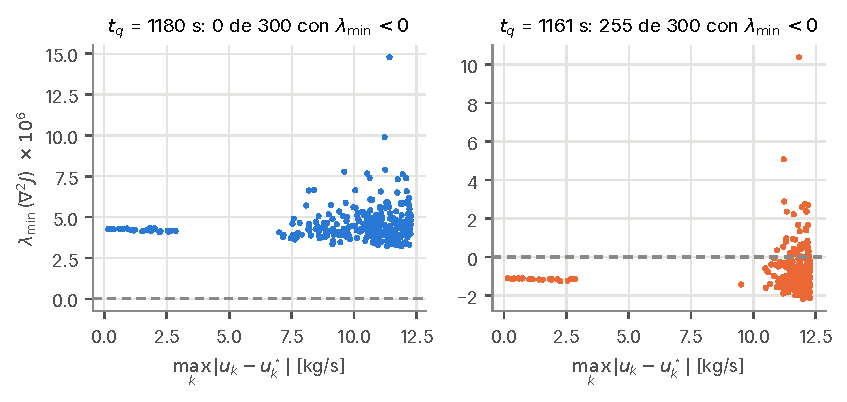
\includegraphics[width=\linewidth]{figures/fig_hessian.pdf}
\caption{Menor valor propio de la hessiana del costo en 300 puntos de la caja de control,
según la distancia a $u^\star$. En 1180~s es positivo en todos: hay señal de convexidad. En
1161~s es levemente negativo en 255 de 300 puntos (hasta $-2\cdot10^{-6}$, un 0.006\,\% de
$\lambda_{\rm max}$), también cerca del óptimo. Eso no contradice el paso 1: en 1161~s las 26
variables están en su cota con multiplicadores positivos, y la dirección de curvatura
negativa queda bloqueada por las cotas.}
\label{fig:hess}
\end{figure}

\noindent La evidencia es fuerte: un solo óptimo en $\approx590$ arranques y ninguna
búsqueda global lo mejora. Pero no es una prueba, y la no convexidad de 1161~s muestra que no
se puede suponer convexidad. Por eso hace falta el paso 4.

\subsection{Paso 4a: cota inferior semi-rigurosa}
\begin{enumerate}
  \item \textbf{Modelo afín de referencia:} $a(u)=\hat y(u_c)+G\,(u-u_c)$, con
        $G=\partial\hat y/\partial u$ exacta en un punto $u_c$. Es sólo una herramienta:
        cualquier modelo afín sirve.
  \item \textbf{Residuo no lineal:} $e_k(u)=\hat y_k(u)-a_k(u)$, con
        $\varepsilon_k\ge\max_{u\in\mathcal U}|e_k(u)|$ estimado por muestreo (3000
        puntos y 63 patrones extremos) y maximización adversaria con Ipopt.
  \item \textbf{Relajación convexa:} si $|e_k|\le\varepsilon_k$, entonces
        $(\hat y_k-y_{\rm ref})^2\ge\big(|a_k(u)-y_{\rm ref}|-\varepsilon_k\big)_+^2$ y
        $[\hat y_k-U_y]_+^2\ge[a_k-\varepsilon_k-U_y]_+^2$. La penalización de la rampa es
        exacta. La función resultante $L(u)$ cumple $L\le J$ en toda la caja y es
        convexa, así que $LB=\min L$ es un QP (Clarabel, cota dual).
\end{enumerate}
Con $u_c=u^\star$, la búsqueda adversaria no supera al muestreo en ningún paso, y la brecha
$(UB-LB)/UB$ es de \textbf{0.30\,\% (1180~s) y 1.2\,\% (1161~s)}. Con un factor de
seguridad de 2 sobre $\varepsilon$ sube a 0.59\,\% y 2.4\,\%. Es \emph{semi}-rigurosa
porque el muestreo podría no encontrar el peor residuo. En sub-cajas de semiancho $\rho$ la
brecha baja como $\rho^2$, igual que el resto de Taylor (figura~\ref{fig:bounds}, derecha).

\subsection{Paso 4b: cota inferior certificada}
Se reemplaza el $\varepsilon$ muestreado por uno \textbf{demostrado}. Para eso se usa un
modelo de Taylor de primer orden con resto por intervalos, en variables escaladas:
\[
\delta_k(u)=x_k(u)-x^c_k=T_k\,\Delta u+r_k,\qquad \Delta u=u-u_c,
\]
donde $r_k$ es una caja de intervalos.
\begin{itemize}
  \item Restando el paso implícito real y el nominal, y aplicando el teorema del valor medio
        a $f$:
        \[
        M_k^c\,r_k=r_{k-1}+h\big([A](Z_k)-A^c_k\big)[\delta_k]-\mathrm{res}_k-D_k\,\Delta u,
        \]
        con $M_k^c=I-hA^c_k$.
        $[A](Z_k)$ es el jacobiano de $f$ evaluado con aritmética de intervalos
        (\code{IntervalArithmetic.jl}) sobre la caja alcanzable $Z_k$. $B=e_{\Delta M}$ es
        constante, porque el control sólo entra en el inventario.
  \item $\mathrm{res}_k$ y $D_k$ son los defectos de punto flotante de la trayectoria
        nominal y de la parte lineal, encerrados con intervalos: el redondeo queda
        controlado.
  \item Como $r_k$ aparece a ambos lados, se acepta una caja $R$ cuando el operador la
        manda dentro de sí misma (teorema de Brouwer). Se supone que cada paso implícito
        tiene solución única, lo que respalda la convergencia de Newton.
  \item El término directo de la salida se acota exactamente:
        $\tfrac12[p_4''](\cdot)\,\Delta u_k^2$.
\end{itemize}

\noindent\emph{Verificaciones.} El jacobiano por intervalos contiene los 1300 jacobianos
muestreados por consulta, sin ninguna violación. La propagación cierra en los 26 pasos (dos
iteraciones de punto fijo por paso, unos 4~s). El $\varepsilon$ riguroso queda por encima del
residuo muestreado del \emph{mismo} modelo afín en todos los pasos.

\begin{table}[H]\centering\small
\begin{tabular}{@{}lccc@{}}\toprule
Centro $u_c$ del modelo de Taylor & $\varepsilon_{26}$ riguroso / muestreado & Brecha 1180~s & Brecha 1161~s\\\midrule
$u^\star$ (solución del NLP) & 0.50 / 0.010~K; 1.32 / 0.038~K & 4.86\,\% & 20.85\,\%\\
Punto medio de la caja & 0.47 / 0.009~K; 0.48 / 0.010~K & \textbf{2.34\,\%} & \textbf{11.44\,\%}\\\bottomrule
\end{tabular}
\caption{Brecha certificada $(UB-LB)/UB$ del P0 no lineal sobre toda la caja de control.
Con el centro en el punto medio, $LB=0.23834$ (1180~s) y $42.533$ (1161~s).}
\end{table}

\begin{figure}[H]\centering
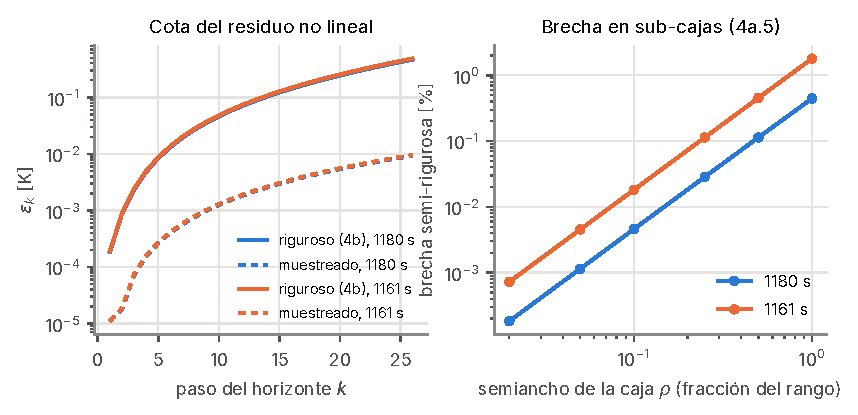
\includegraphics[width=\linewidth]{figures/fig_bounds.pdf}
\caption{Izquierda: cota del residuo no lineal por paso del horizonte, rigurosa (4b) frente a
muestreada, con el modelo centrado en el punto medio. Derecha: brecha semi-rigurosa en
sub-cajas de semiancho $\rho$ alrededor de $u^\star$ (4a.5), que baja como $\rho^2$.}
\label{fig:bounds}
\end{figure}

\takeaway{\textbf{Lectura.} Es la \textbf{primera cota inferior certificada} del P0 no
lineal: el óptimo global está en $[0.23834,\ 0.24403]$ (1180~s) y en $[42.53,\ 48.03]$
(1161~s). El $\varepsilon$ riguroso sobreestima el real entre 16 y 50 veces, por dos
razones. (i) El término de segundo orden se acota como el producto de dos cajas, lo que
ignora que las 26 direcciones de control mueven el estado casi en una sola dirección, la del
inventario. (ii) El resto se acumula a través del integrador. El ajuste (paso 4b.5: partición
por masa inyectada o modelo de Taylor de segundo orden) queda para la próxima ronda.}

\section{Comparación de las decisiones de todos los métodos}\label{sec:comparacion}

\subsection{Modelos y métodos comparados}
Cada método entrega una secuencia de 26 caudales del ACS para la misma consulta. Lo que
cambia es el modelo con que decide, la formulación y el algoritmo:

\begin{table}[H]\centering\footnotesize\setlength{\tabcolsep}{3pt}
\begin{tabularx}{\linewidth}{@{}>{\raggedright\arraybackslash}p{24mm} Y Y Y r@{}}\toprule
Método & Modelo con el que decide & Formulación & Algoritmo y derivadas & Tiempo\\\midrule
N3, NLP (BE) & ROM no lineal, Euler implícito convergido & Monolítica dispersa: 519 variables, 442 igualdades & Ipopt (punto interior), hessiana exacta por diferenciación automática & 0.05~s\\
N3 sobre \code{ode1be} & ROM no lineal, \code{ode1be} (= Simulink) & Espacio reducido: 26 variables & Ipopt, gradiente exacto a través de la simulación, hessiana L-BFGS & 2.5--10~s\\
N2, QP-LTV iterado & ROM linealizado en cada paso de la trayectoria del incumbente & QP condensado (77 variables) por iteración & SQP: simular, linealizar (ForwardDiff), QP (Clarabel); 4 iteraciones en 1180~s, 1 en 1161~s & $\sim$10~ms por QP\\
N1, QP-LTI & ROM linealizado en el punto de consulta & QP condensado, 77 variables & Clarabel, con certificado dual & 0.01~s\\
Evolución diferencial & ROM no lineal, Euler implícito & 26 variables & Sin derivadas: DE/rand/1/bin, 90\,060 evaluaciones & 90~s\\
LJ corregido & ROM en Simulink (\code{DET\_2} + \code{fitness\_cost}) & 26 corrientes & Sin derivadas: Luus--Jaakola ($R=24$, $\gamma=0.9$, $M=5$), 721 evaluaciones & $\approx800$~s\\
GA & Igual que LJ & 26 corrientes & Sin derivadas: genético $20\times20$, cruce 0.8, mutación 0.3, 420 evaluaciones & $\approx615$~s\\
Lazo archivado & Lazo original, anterior a la corrección de LJ & --- & --- & ---\\\bottomrule
\end{tabularx}
\caption{Métodos comparados. Los tiempos de LJ y GA se midieron en MATLAB/Simulink (E2); los
demás, en Julia sobre leo\_acer.}
\end{table}

\subsection{Consideraciones para que la comparación sea justa}
\begin{enumerate}
  \item \textbf{Misma vara.} Cada control se evalúa con el costo P0 sobre el ROM \emph{no
        lineal}, en las dos discretizaciones (Euler implícito y \code{ode1be}). Las dos dan
        el mismo ordenamiento, y difieren en un desplazamiento casi constante de
        $3.6\cdot10^{-5}$ (1180~s). Las corrientes de LJ y GA se convierten a caudal con el
        mapa de la bomba. Su costo recalculado coincide con el que E2 midió en Simulink
        (por ejemplo, 4.081 para el LJ archivado).
  \item \textbf{Mismas condiciones.} Todos parten del mismo estado $x(t_q-\Delta t)$ y usan
        el mismo pronóstico de fuga (el de F2), la misma referencia, las mismas cotas
        archivadas del actuador (0.58--12.86~kg/s) y la rampa blanda de P0.
  \item \textbf{Cómo se mide la calidad.} Se usa el costo no lineal de cada decisión, nunca el
        objetivo interno de su solver. Por ejemplo, el QP N1 predice 47.81 en 1161~s, pero su
        control cuesta 48.03 en el modelo no lineal: el 47.81 no es una cota de nada.
  \item \textbf{Exceso garantizado.} Como $LB\le J^\star\le UB$, el exceso real de una
        decisión $u$ sobre el óptimo global queda en el intervalo
        $\big[(J(u)-UB)/UB,\ (J(u)-LB)/LB\big]$. El extremo inferior es el exceso sobre el
        mejor encontrado; el superior, la peor posibilidad compatible con la cota certificada.
  \item \textbf{Alcance.} La comparación vale para P0 sobre el ROM, en dos consultas y con las
        cotas archivadas del actuador, que no tienen base física
        (sección~\ref{sec:f3c}). No dice nada sobre el desajuste ROM--HRM. En 1161~s, LJ y GA
        no tienen corridas completas.
\end{enumerate}

\subsection{Resultados}

\begin{table}[H]\centering\footnotesize\setlength{\tabcolsep}{3pt}
\begin{tabular}{@{}lrrrrr@{}}\toprule
& \multicolumn{3}{c}{$t_q=1180$~s} & \multicolumn{2}{c}{$t_q=1161$~s}\\
\cmidrule(lr){2-4}\cmidrule(l){5-6}
Método & Costo & Exceso/mejor & Exceso garantizado & Costo & Exceso/mejor\\\midrule
N3, NLP (Ipopt, BE) & 0.244034 & 0 & 0 -- 2.4\,\% & 48.028 & 0\\
N3 sobre \code{ode1be} & 0.244034 & 0 & 0 -- 2.4\,\% & 48.028 & 0\\
N2, QP-LTV iterado & 0.244034 & 0 & 0 -- 2.4\,\% & 48.028 & 0\\
N1, QP-LTI & 0.244040 & +0.0026\,\% & 0.0026 -- 2.4\,\% & 48.028 & 0\\
Evolución diferencial & 0.244034 & +0.0001\,\% & 0.0001 -- 2.4\,\% & 48.028 & 0\\
LJ corregido (3 semillas) & 0.313 -- 0.381 & +28 a +56\,\% & 28 -- 60\,\% & --- & ---\\
GA (2 semillas) & 0.349 -- 0.353 & +43 a +45\,\% & 43 -- 48\,\% & --- & ---\\
Lazo archivado & 4.081 & +1572\,\% & 1572 -- 1612\,\% & 94.45 & +97\,\%\\\bottomrule
\end{tabular}
\caption{Costo P0 sobre el ROM no lineal (Euler implícito) de la decisión de cada método. En
1161~s el exceso garantizado de N1--N3 y DE es 0--12.9\,\%, y el del lazo archivado,
97--122\,\%.}
\end{table}

\begin{figure}[H]\centering
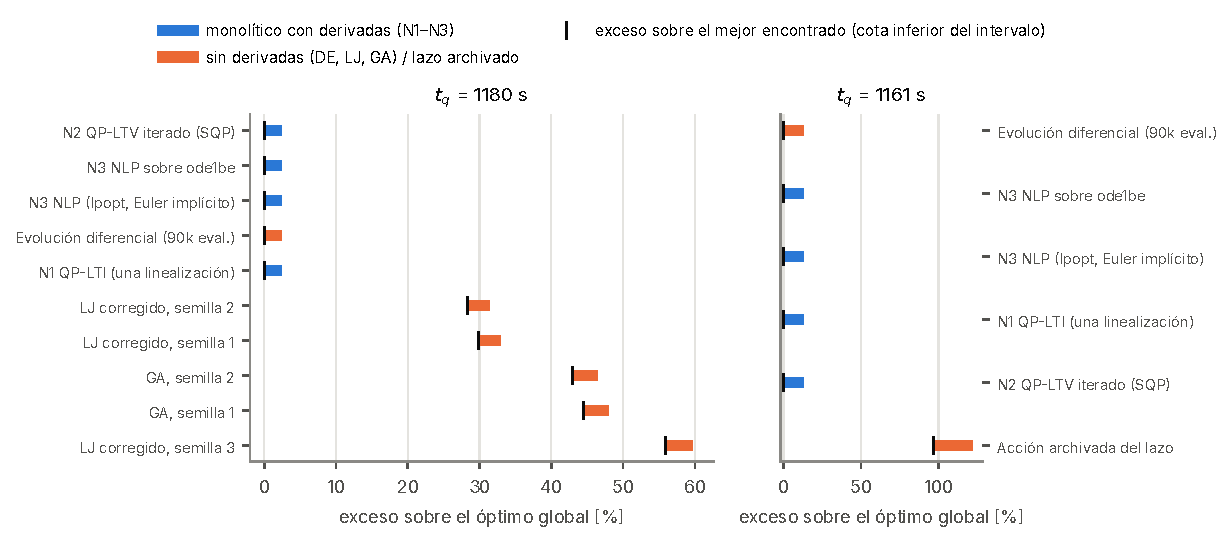
\includegraphics[width=\linewidth]{figures/fig_decisions.pdf}
\caption{Intervalo de exceso garantizado sobre el óptimo global de cada decisión. La marca
negra es el exceso sobre el mejor encontrado (extremo inferior) y la barra llega hasta el
extremo superior, que fija la cota certificada. En 1180~s se omite el lazo archivado (1572--1612\,\%).}
\end{figure}

\takeaway{\textbf{Conclusiones.} (i) \textbf{N3 y N2 son los mejores y empatan}: son la
misma decisión, a $6\cdot10^{-6}$~kg/s. (ii) \textbf{N1} cuesta un 0.0026\,\% más en 1180~s
y lo mismo en 1161~s. Es el más rápido ($\sim$10~ms) y el único que es un QP convexo
certificable, así que es el candidato natural para tiempo real. (iii) La primera acción
aplicada (56.75~A) coincide en N1, N2, N3 y DE. LJ con la semilla 3 y las dos semillas de GA
aplican otra. (iv) \textbf{LJ y GA quedan dominados con garantía}: su exceso sobre el óptimo
global es de al menos 28\,\% y 43\,\%, y son unas $10^4$ veces más lentos. (v) El límite
superior del intervalo de N1--N3 (2.4\,\%) es la brecha de la cota certificada, no una
pérdida observada: los pasos 1--3 indican que el exceso real es $\approx0$. Cerrarlo es el
paso 4b.5.}

\section{Estado actual}

\begin{itemize}
  \item \textbf{Herramientas.} Toda la cadena F1--F4 corre sin MATLAB en Julia
        (\code{julia/SMDFRROM.jl} y \code{F4Lib.jl}) y en Python con \code{torch} en CPU.
        MATLAB (leo\_asus) sólo hace falta para generar consultas nuevas, el HRM y el lazo
        completo.
  \item \textbf{Resuelto.} El MPC determinista es tratable y reproducible: el NLP tarda
        unos 0.05~s y el QP condensado unos 10~ms por consulta. El QP tiene certificado
        dual de optimalidad global para su modelo lineal, y N2 converge al NLP: son dos
        verificaciones independientes del óptimo local. El SAA con 59 escenarios toma unos
        2~s, así que la capa 2 de riesgo es viable en tiempo real.
  \item \textbf{Certificación del P0 no lineal (F3c).} La solución de Ipopt es un mínimo
        local estricto y el único óptimo encontrado en $\approx590$ arranques y en una
        búsqueda global sin derivadas. La primera brecha \emph{certificada} es de 2.3\,\%
        (1180~s) y 11.4\,\% (1161~s); la semi-rigurosa, de 0.3\,\% y 1.2\,\%. En la
        comparación con la misma vara, N3 y N2 empatan como los mejores, N1 queda a
        0.0026\,\%, y LJ y GA quedan al menos un 28\,\% y un 43\,\% por encima del óptimo
        global.
  \item \textbf{Abierto.} La brecha certificada es conservadora (paso 4b.5). F4 todavía no
        tiene ``una decisión que cambie por riesgo''. Las conclusiones se apoyan en dos
        consultas, y la cota del actuador no está fijada.
\end{itemize}

\section{Próximos pasos}

\begin{enumerate}
  \item \textbf{Fijar el actuador con el equipo:} la rampa admisible, el caudal máximo y
        si el ACS repone inventario o impulsa el caudal primario. Es la decisión que más
        cambia los resultados: el costo óptimo en 1161~s va de 3.1 a 48.4. No requiere
        ninguna máquina.
  \item \textbf{F4 con escenarios de falla del ACS} (leo\_acer): SAA o MPC multietapa con
        no anticipación sobre el modo $\sigma\in\{0,1\}$ y las tasas $\lambda,\mu$ del DET.
        Criterio: una primera acción que cambie por riesgo, con intervalo de confianza.
  \item \textbf{Desajuste ROM--HRM como incertidumbre} (leo\_asus): re-simular en el HRM
        las acciones del NLP. Si el error es del orden de 1~K, es la incertidumbre que
        corresponde a la restricción probabilística.
  \item \textbf{Recalibrar el pronóstico} (leo\_acer): corregir el sesgo, por ejemplo con
        un modelo de error o predicción conformal, y usar \code{N\_par}~$>1$ en el lazo.
  \item \textbf{Más consultas} (leo\_asus): reconstruir varias de las 61 con
        \code{build\_query\_from\_archive.m}.
  \item \textbf{F5, lazo cerrado} (leo\_asus): las 61 consultas con el NLP o el QP frente
        al lazo LJ archivado, con menos de 120~s por consulta.
  \item \textbf{F3c, paso 4b.5} (leo\_acer, próxima ronda): ajustar la cota certificada con
        una partición por masa inyectada o un modelo de Taylor de segundo orden. El objetivo
        es cerrar el exceso garantizado de N1--N3 (hoy 0--2.4\,\% y 0--12.9\,\%) hacia los
        valores semi-rigurosos (0.3\,\% y 1.2\,\%).
\end{enumerate}

\paragraph{Reproducibilidad.}
\begin{itemize}\sloppy
  \item Resultados: \code{results/f1\_rom\_replica/}, \code{results/f3\_certificates/},
        \code{results/f3c\_optimality/} y \code{results/f4\_risk/}.
  \item Julia: \code{julia/f2\_monolithic\_nlp.jl}, \code{f3\_certificates\_condensed.jl}
        (sustituye a \code{f3\_linearized\_qp.jl}), \code{f3c\_optimality.jl} (pasos 1--3),
        \code{f3c\_lower\_bound.jl} (4a), \code{f3c\_rigorous.jl} (4b; centro con
        \code{F3C\_CENTER=mid}), \code{f3c\_compare\_decisions.jl}, \code{ReducedP0.jl},
        \code{f4\_risk\_decisions.jl} y \code{f4\_actuator\_sweep.jl}.
  \item Python: \code{python/f4\_leak\_ensemble.py}, \code{f4\_forecast\_calibration.py}
        y \code{make\_status\_figures.py} (figuras).
\end{itemize}

\end{document}
